\documentclass[11pt, a4paper]{article}\usepackage[]{graphicx}\usepackage[]{xcolor}
% maxwidth is the original width if it is less than linewidth
% otherwise use linewidth (to make sure the graphics do not exceed the margin)
\makeatletter
\def\maxwidth{ %
  \ifdim\Gin@nat@width>\linewidth
    \linewidth
  \else
    \Gin@nat@width
  \fi
}
\makeatother

\definecolor{fgcolor}{rgb}{0.345, 0.345, 0.345}
\newcommand{\hlnum}[1]{\textcolor[rgb]{0.686,0.059,0.569}{#1}}%
\newcommand{\hlsng}[1]{\textcolor[rgb]{0.192,0.494,0.8}{#1}}%
\newcommand{\hlcom}[1]{\textcolor[rgb]{0.678,0.584,0.686}{\textit{#1}}}%
\newcommand{\hlopt}[1]{\textcolor[rgb]{0,0,0}{#1}}%
\newcommand{\hldef}[1]{\textcolor[rgb]{0.345,0.345,0.345}{#1}}%
\newcommand{\hlkwa}[1]{\textcolor[rgb]{0.161,0.373,0.58}{\textbf{#1}}}%
\newcommand{\hlkwb}[1]{\textcolor[rgb]{0.69,0.353,0.396}{#1}}%
\newcommand{\hlkwc}[1]{\textcolor[rgb]{0.333,0.667,0.333}{#1}}%
\newcommand{\hlkwd}[1]{\textcolor[rgb]{0.737,0.353,0.396}{\textbf{#1}}}%
\let\hlipl\hlkwb

\usepackage{framed}
\makeatletter
\newenvironment{kframe}{%
 \def\at@end@of@kframe{}%
 \ifinner\ifhmode%
  \def\at@end@of@kframe{\end{minipage}}%
  \begin{minipage}{\columnwidth}%
 \fi\fi%
 \def\FrameCommand##1{\hskip\@totalleftmargin \hskip-\fboxsep
 \colorbox{shadecolor}{##1}\hskip-\fboxsep
     % There is no \\@totalrightmargin, so:
     \hskip-\linewidth \hskip-\@totalleftmargin \hskip\columnwidth}%
 \MakeFramed {\advance\hsize-\width
   \@totalleftmargin\z@ \linewidth\hsize
   \@setminipage}}%
 {\par\unskip\endMakeFramed%
 \at@end@of@kframe}
\makeatother

\definecolor{shadecolor}{rgb}{.97, .97, .97}
\definecolor{messagecolor}{rgb}{0, 0, 0}
\definecolor{warningcolor}{rgb}{1, 0, 1}
\definecolor{errorcolor}{rgb}{1, 0, 0}
\newenvironment{knitrout}{}{} % an empty environment to be redefined in TeX

\usepackage{alltt}

\usepackage[top=1 in, bottom = 1 in, left = 1 in, right = 1 in ]{geometry}

\usepackage{amsmath, amssymb, amsfonts}
\usepackage{enumerate}
\usepackage{dingbat}
\usepackage{fontawesome5}
\usepackage{twemojis}

\title{MSMS 106}
\author{Ananda Biswas}
\date{}
\IfFileExists{upquote.sty}{\usepackage{upquote}}{}
\begin{document}

\maketitle

\begin{center}
\textbf{Practical 05}
\end{center}

\scalebox{2.0}{\twemoji{bullseye}} \hspace{0.2cm} \textcolor{blue}{\textbf{Polynomial Approximation}}

\vspace{0.5cm}

\smallpencil \hspace{0.2cm} Find a linear fit to the following data.

\begin{table}[!htbp]
\def\arraystretch{1.5}

\begin{center}
\begin{tabular}{|c|c|c|c|c|c|}

\hline

$x$ & 1 & 2 & 3 & 4 & 5 \\

\hline

$f(x)$ & 1.2 & 2.3 & 2.9 & 4.1 & 5.2 \\

\hline
\end{tabular}
\end{center}

\end{table}

\faArrowAltCircleRight[regular] \hspace{0.2cm} Let $f(x) \approx P_1(x) = a_0 + a_1 x$.

\begin{knitrout}
\definecolor{shadecolor}{rgb}{0.969, 0.969, 0.969}\color{fgcolor}\begin{kframe}
\begin{alltt}
\hldef{df1} \hlkwb{<-} \hlkwd{data.frame}\hldef{(}\hlkwc{x} \hldef{=} \hlnum{1}\hlopt{:}\hlnum{5}\hldef{,}
                  \hlkwc{y} \hldef{=} \hlkwd{c}\hldef{(}\hlnum{1.2}\hldef{,} \hlnum{2.3}\hldef{,} \hlnum{2.9}\hldef{,} \hlnum{4.1}\hldef{,} \hlnum{5.2}\hldef{))}
\end{alltt}
\end{kframe}
\end{knitrout}

\begin{knitrout}
\definecolor{shadecolor}{rgb}{0.969, 0.969, 0.969}\color{fgcolor}\begin{kframe}
\begin{alltt}
\hldef{fit1} \hlkwb{<-} \hlkwd{lm}\hldef{(y} \hlopt{~} \hldef{x,} \hlkwc{data} \hldef{= df1)}
\hldef{fit1}\hlopt{$}\hldef{coefficients}
\end{alltt}
\begin{verbatim}
## (Intercept)           x 
##        0.20        0.98
\end{verbatim}
\end{kframe}
\end{knitrout}

So, $P_1(x) = 0.2 + 0.98 x$.



\begin{knitrout}
\definecolor{shadecolor}{rgb}{0.969, 0.969, 0.969}\color{fgcolor}\begin{kframe}
\begin{alltt}
\hldef{df1} \hlopt
  \hlkwd{ggplot}\hldef{(}\hlkwd{aes}\hldef{(}\hlkwc{x} \hldef{= x,} \hlkwc{y} \hldef{= y))} \hlopt{+}
  \hlkwd{geom_point}\hldef{(}\hlkwc{col} \hldef{=} \hlsng{"red"}\hldef{,} \hlkwc{size} \hldef{=} \hlnum{3}\hldef{)} \hlopt{+}
  \hlkwd{geom_smooth}\hldef{(}\hlkwc{method} \hldef{=} \hlsng{"lm"}\hldef{,} \hlkwc{formula} \hldef{= y} \hlopt{~} \hldef{x,} \hlkwc{se} \hldef{=} \hlnum{FALSE}\hldef{)} \hlopt{+}
  \hlkwd{labs}\hldef{(}\hlkwc{title} \hldef{=} \hlsng{"Fitting a linear polynomial"}\hldef{)}
\end{alltt}
\end{kframe}
\end{knitrout}



\begin{knitrout}
\definecolor{shadecolor}{rgb}{0.969, 0.969, 0.969}\color{fgcolor}\begin{kframe}
\begin{alltt}
\hldef{fit1_residuals} \hlkwb{<-} \hlkwd{data.frame}\hldef{(}\hlkwc{index} \hldef{=} \hlnum{1}\hlopt{:}\hlnum{5}\hldef{,} \hlkwc{residual} \hldef{= fit1}\hlopt{$}\hldef{residuals)}

\hldef{fit1_residuals} \hlopt
  \hlkwd{ggplot}\hldef{(}\hlkwd{aes}\hldef{(}\hlkwc{x} \hldef{= index,} \hlkwc{y} \hldef{= residual))} \hlopt{+}
  \hlkwd{geom_point}\hldef{(}\hlkwc{col} \hldef{=} \hlsng{"red"}\hldef{,} \hlkwc{size} \hldef{=} \hlnum{3}\hldef{)} \hlopt{+}
  \hlkwd{geom_hline}\hldef{(}\hlkwc{yintercept} \hldef{=} \hlnum{0}\hldef{,} \hlkwc{col} \hldef{=} \hlsng{"blue"}\hldef{,} \hlkwc{linewidth} \hldef{=} \hlnum{1}\hldef{)} \hlopt{+}
  \hlkwd{labs}\hldef{(}\hlkwc{title} \hldef{=} \hlsng{"Residual Plot"}\hldef{)}
\end{alltt}
\end{kframe}
\end{knitrout}



\newpage

\begin{table}[!htbp]
\def\arraystretch{1.5}

\begin{center}

\begin{tabular}{cc}

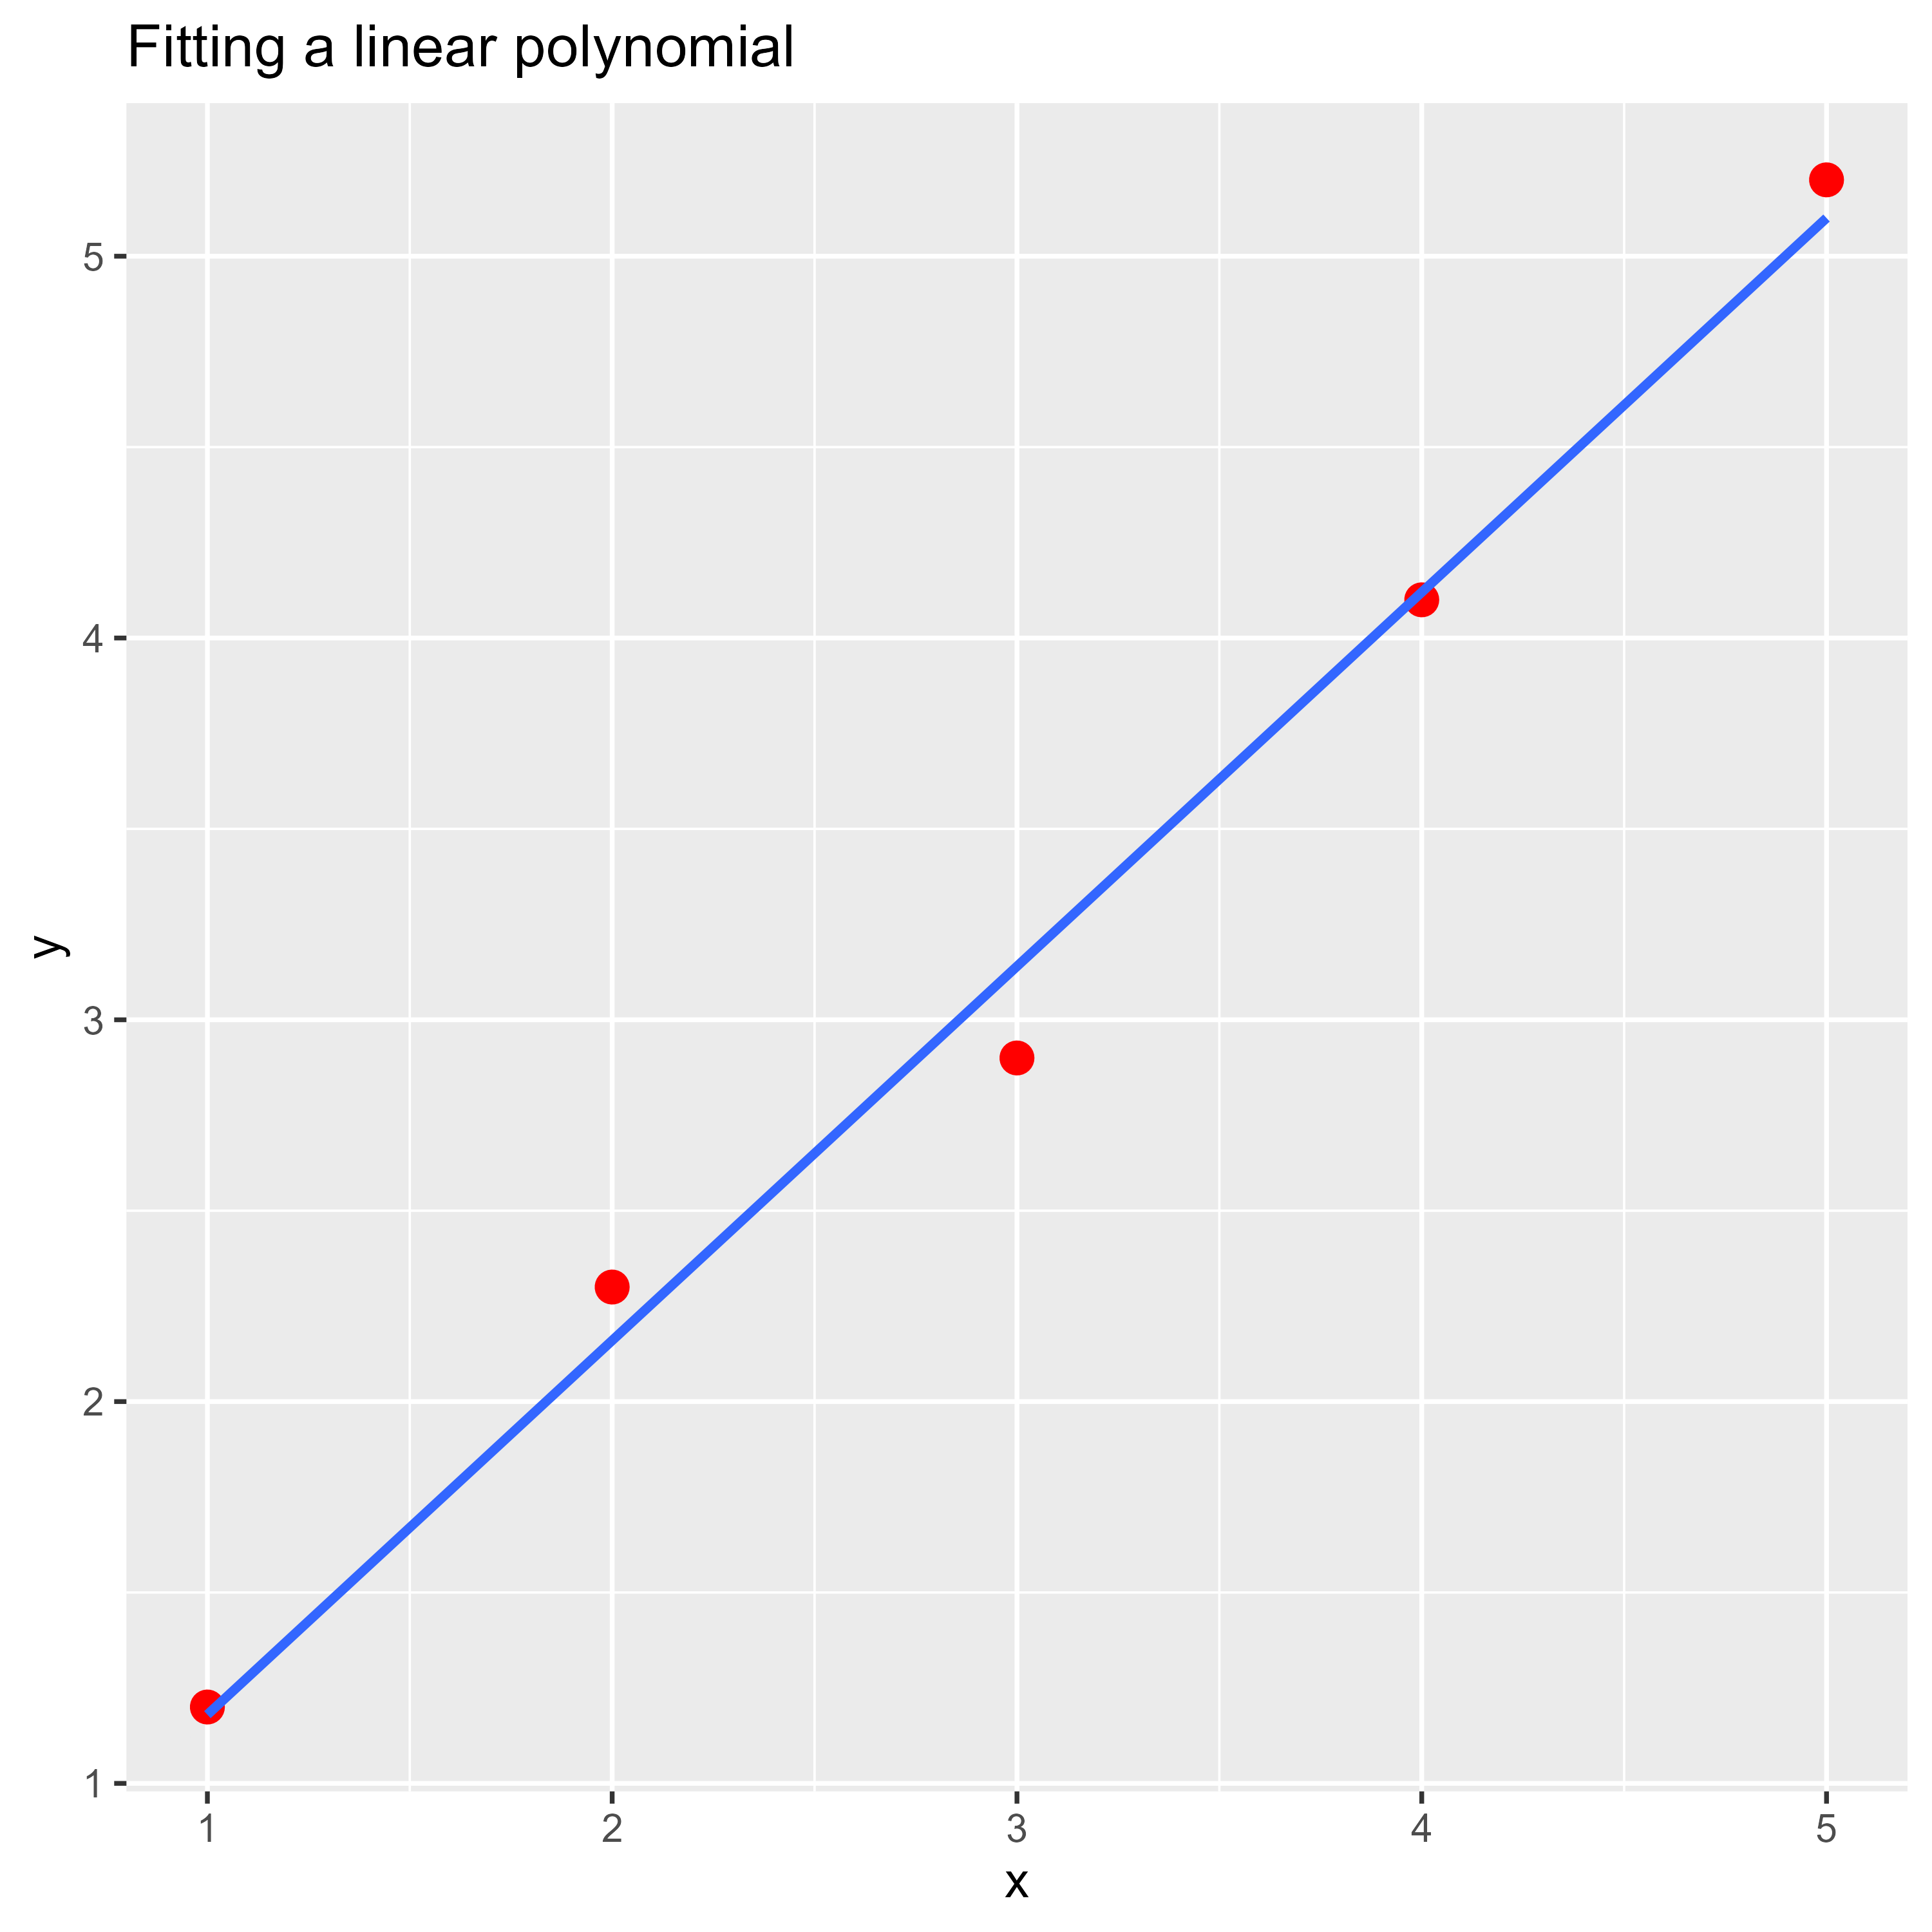
\includegraphics[scale = 0.5]{fit1} & 
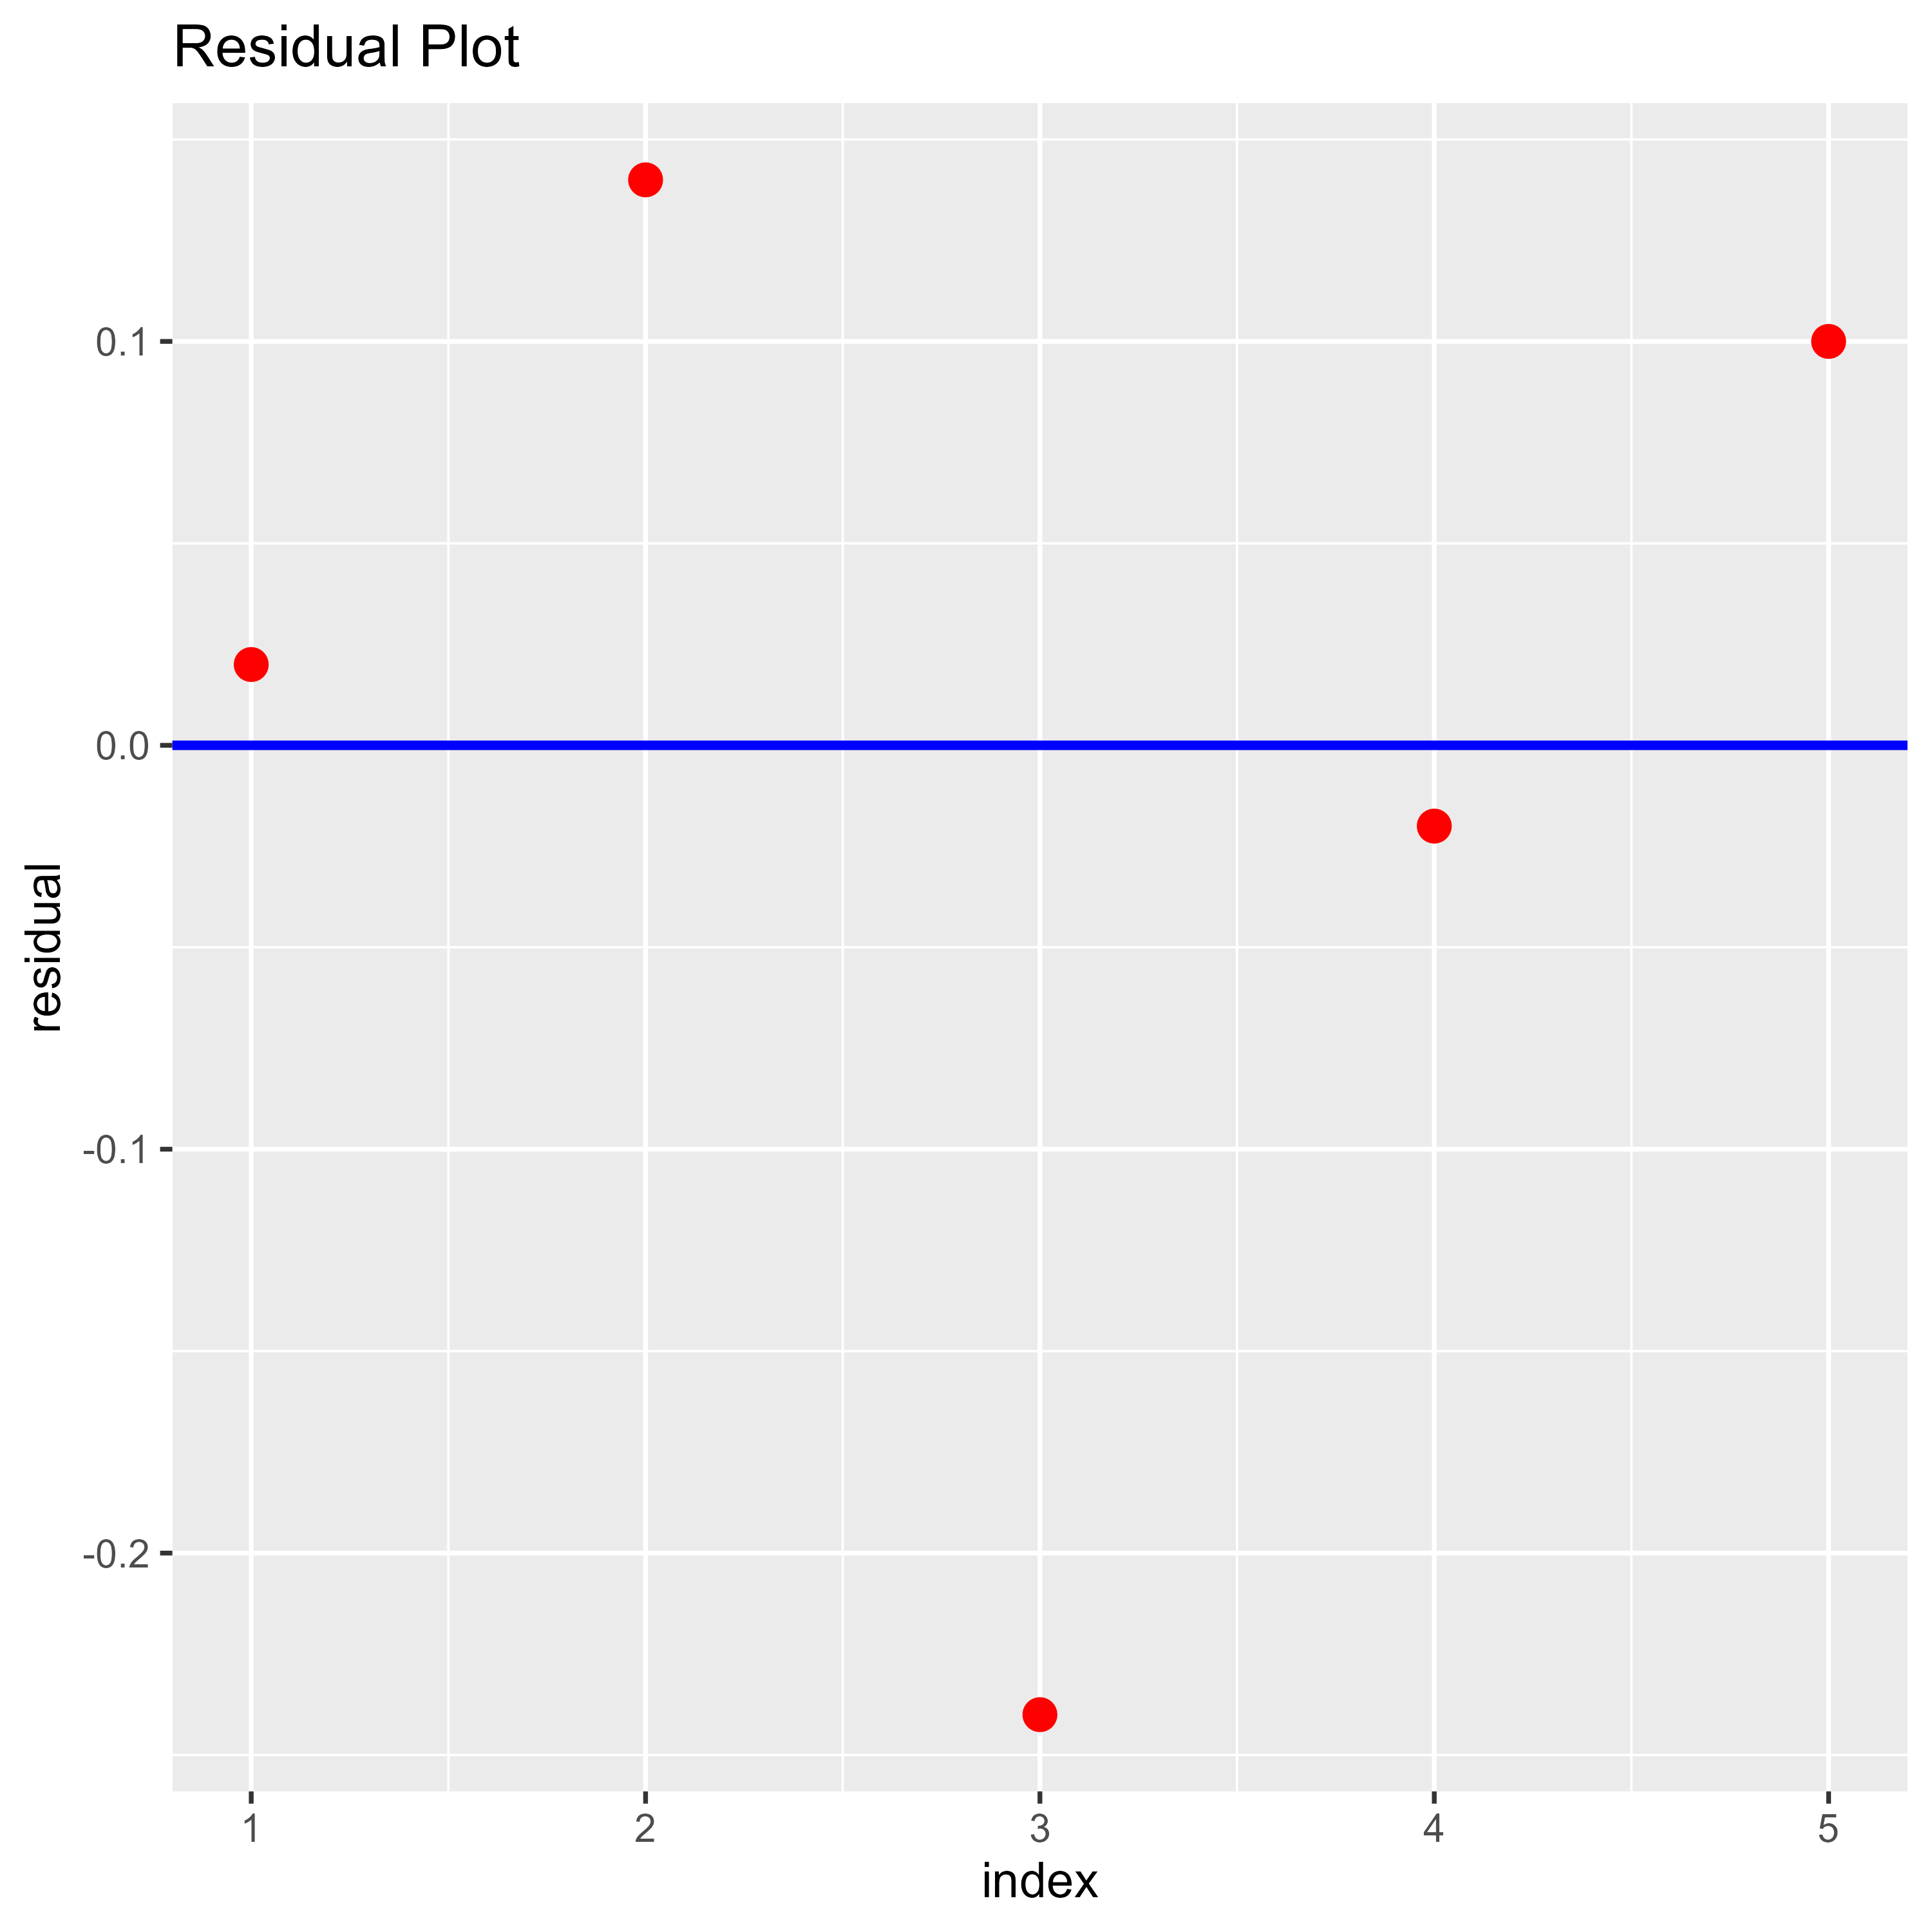
\includegraphics[scale = 0.5]{fit1_residuals}
\end{tabular}
\end{center}
\end{table}


\smallpencil \hspace{0.2cm} Find a linear fit to the following data.

\begin{table}[!htbp]
\def\arraystretch{1.5}

\begin{center}
\begin{tabular}{|c|c|c|c|c|c|}

\hline

$x$ & 0.2 & 0.4 & 0.6 & 0.8 & 1 \\

\hline

$f(x)$ & 0.447 & 0.632 & 0.775 & 0.894 & 1 \\

\hline
\end{tabular}
\end{center}

\end{table}

\faArrowAltCircleRight[regular] \hspace{0.2cm} Let $f(x) \approx P_1(x) = a_0 + a_1 x$.

\begin{knitrout}
\definecolor{shadecolor}{rgb}{0.969, 0.969, 0.969}\color{fgcolor}\begin{kframe}
\begin{alltt}
\hldef{df2} \hlkwb{<-} \hlkwd{data.frame}\hldef{(}\hlkwc{x} \hldef{=} \hlkwd{c}\hldef{(}\hlnum{0.2}\hldef{,} \hlnum{0.4}\hldef{,} \hlnum{0.6}\hldef{,} \hlnum{0.8}\hldef{,} \hlnum{1}\hldef{),}
                  \hlkwc{y} \hldef{=} \hlkwd{c}\hldef{(}\hlnum{0.447}\hldef{,} \hlnum{0.632}\hldef{,} \hlnum{0.775}\hldef{,} \hlnum{0.894}\hldef{,} \hlnum{1}\hldef{))}
\end{alltt}
\end{kframe}
\end{knitrout}

\begin{knitrout}
\definecolor{shadecolor}{rgb}{0.969, 0.969, 0.969}\color{fgcolor}\begin{kframe}
\begin{alltt}
\hldef{fit2} \hlkwb{<-} \hlkwd{lm}\hldef{(y} \hlopt{~} \hldef{x,} \hlkwc{data} \hldef{= df2)}
\hldef{fit2}\hlopt{$}\hldef{coefficients}
\end{alltt}
\begin{verbatim}
## (Intercept)           x 
##      0.3392      0.6840
\end{verbatim}
\end{kframe}
\end{knitrout}

So, $P_1(x) = 0.3392 + 0.684 x$.

\begin{knitrout}
\definecolor{shadecolor}{rgb}{0.969, 0.969, 0.969}\color{fgcolor}\begin{kframe}
\begin{alltt}
\hldef{df2} \hlopt
  \hlkwd{ggplot}\hldef{(}\hlkwd{aes}\hldef{(}\hlkwc{x} \hldef{= x,} \hlkwc{y} \hldef{= y))} \hlopt{+}
  \hlkwd{geom_point}\hldef{(}\hlkwc{col} \hldef{=} \hlsng{"red"}\hldef{,} \hlkwc{size} \hldef{=} \hlnum{3}\hldef{)} \hlopt{+}
  \hlkwd{geom_smooth}\hldef{(}\hlkwc{method} \hldef{=} \hlsng{"lm"}\hldef{,} \hlkwc{formula} \hldef{= y} \hlopt{~} \hldef{x,} \hlkwc{se} \hldef{=} \hlnum{FALSE}\hldef{)} \hlopt{+}
  \hlkwd{labs}\hldef{(}\hlkwc{title} \hldef{=} \hlsng{"Fitting a linear polynomial"}\hldef{)}
\end{alltt}
\end{kframe}
\end{knitrout}



\begin{knitrout}
\definecolor{shadecolor}{rgb}{0.969, 0.969, 0.969}\color{fgcolor}\begin{kframe}
\begin{alltt}
\hldef{fit2_residuals} \hlkwb{<-} \hlkwd{data.frame}\hldef{(}\hlkwc{index} \hldef{=} \hlnum{1}\hlopt{:}\hlnum{5}\hldef{,} \hlkwc{residual} \hldef{= fit2}\hlopt{$}\hldef{residuals)}

\hldef{fit2_residuals} \hlopt
  \hlkwd{ggplot}\hldef{(}\hlkwd{aes}\hldef{(}\hlkwc{x} \hldef{= index,} \hlkwc{y} \hldef{= residual))} \hlopt{+}
  \hlkwd{geom_point}\hldef{(}\hlkwc{col} \hldef{=} \hlsng{"red"}\hldef{,} \hlkwc{size} \hldef{=} \hlnum{3}\hldef{)} \hlopt{+}
  \hlkwd{geom_hline}\hldef{(}\hlkwc{yintercept} \hldef{=} \hlnum{0}\hldef{,} \hlkwc{col} \hldef{=} \hlsng{"blue"}\hldef{,} \hlkwc{linewidth} \hldef{=} \hlnum{1}\hldef{)} \hlopt{+}
  \hlkwd{labs}\hldef{(}\hlkwc{title} \hldef{=} \hlsng{"Residual Plot"}\hldef{)}
\end{alltt}
\end{kframe}
\end{knitrout}



\newpage

\begin{table}[!htbp]
\def\arraystretch{1.5}

\begin{center}

\begin{tabular}{cc}

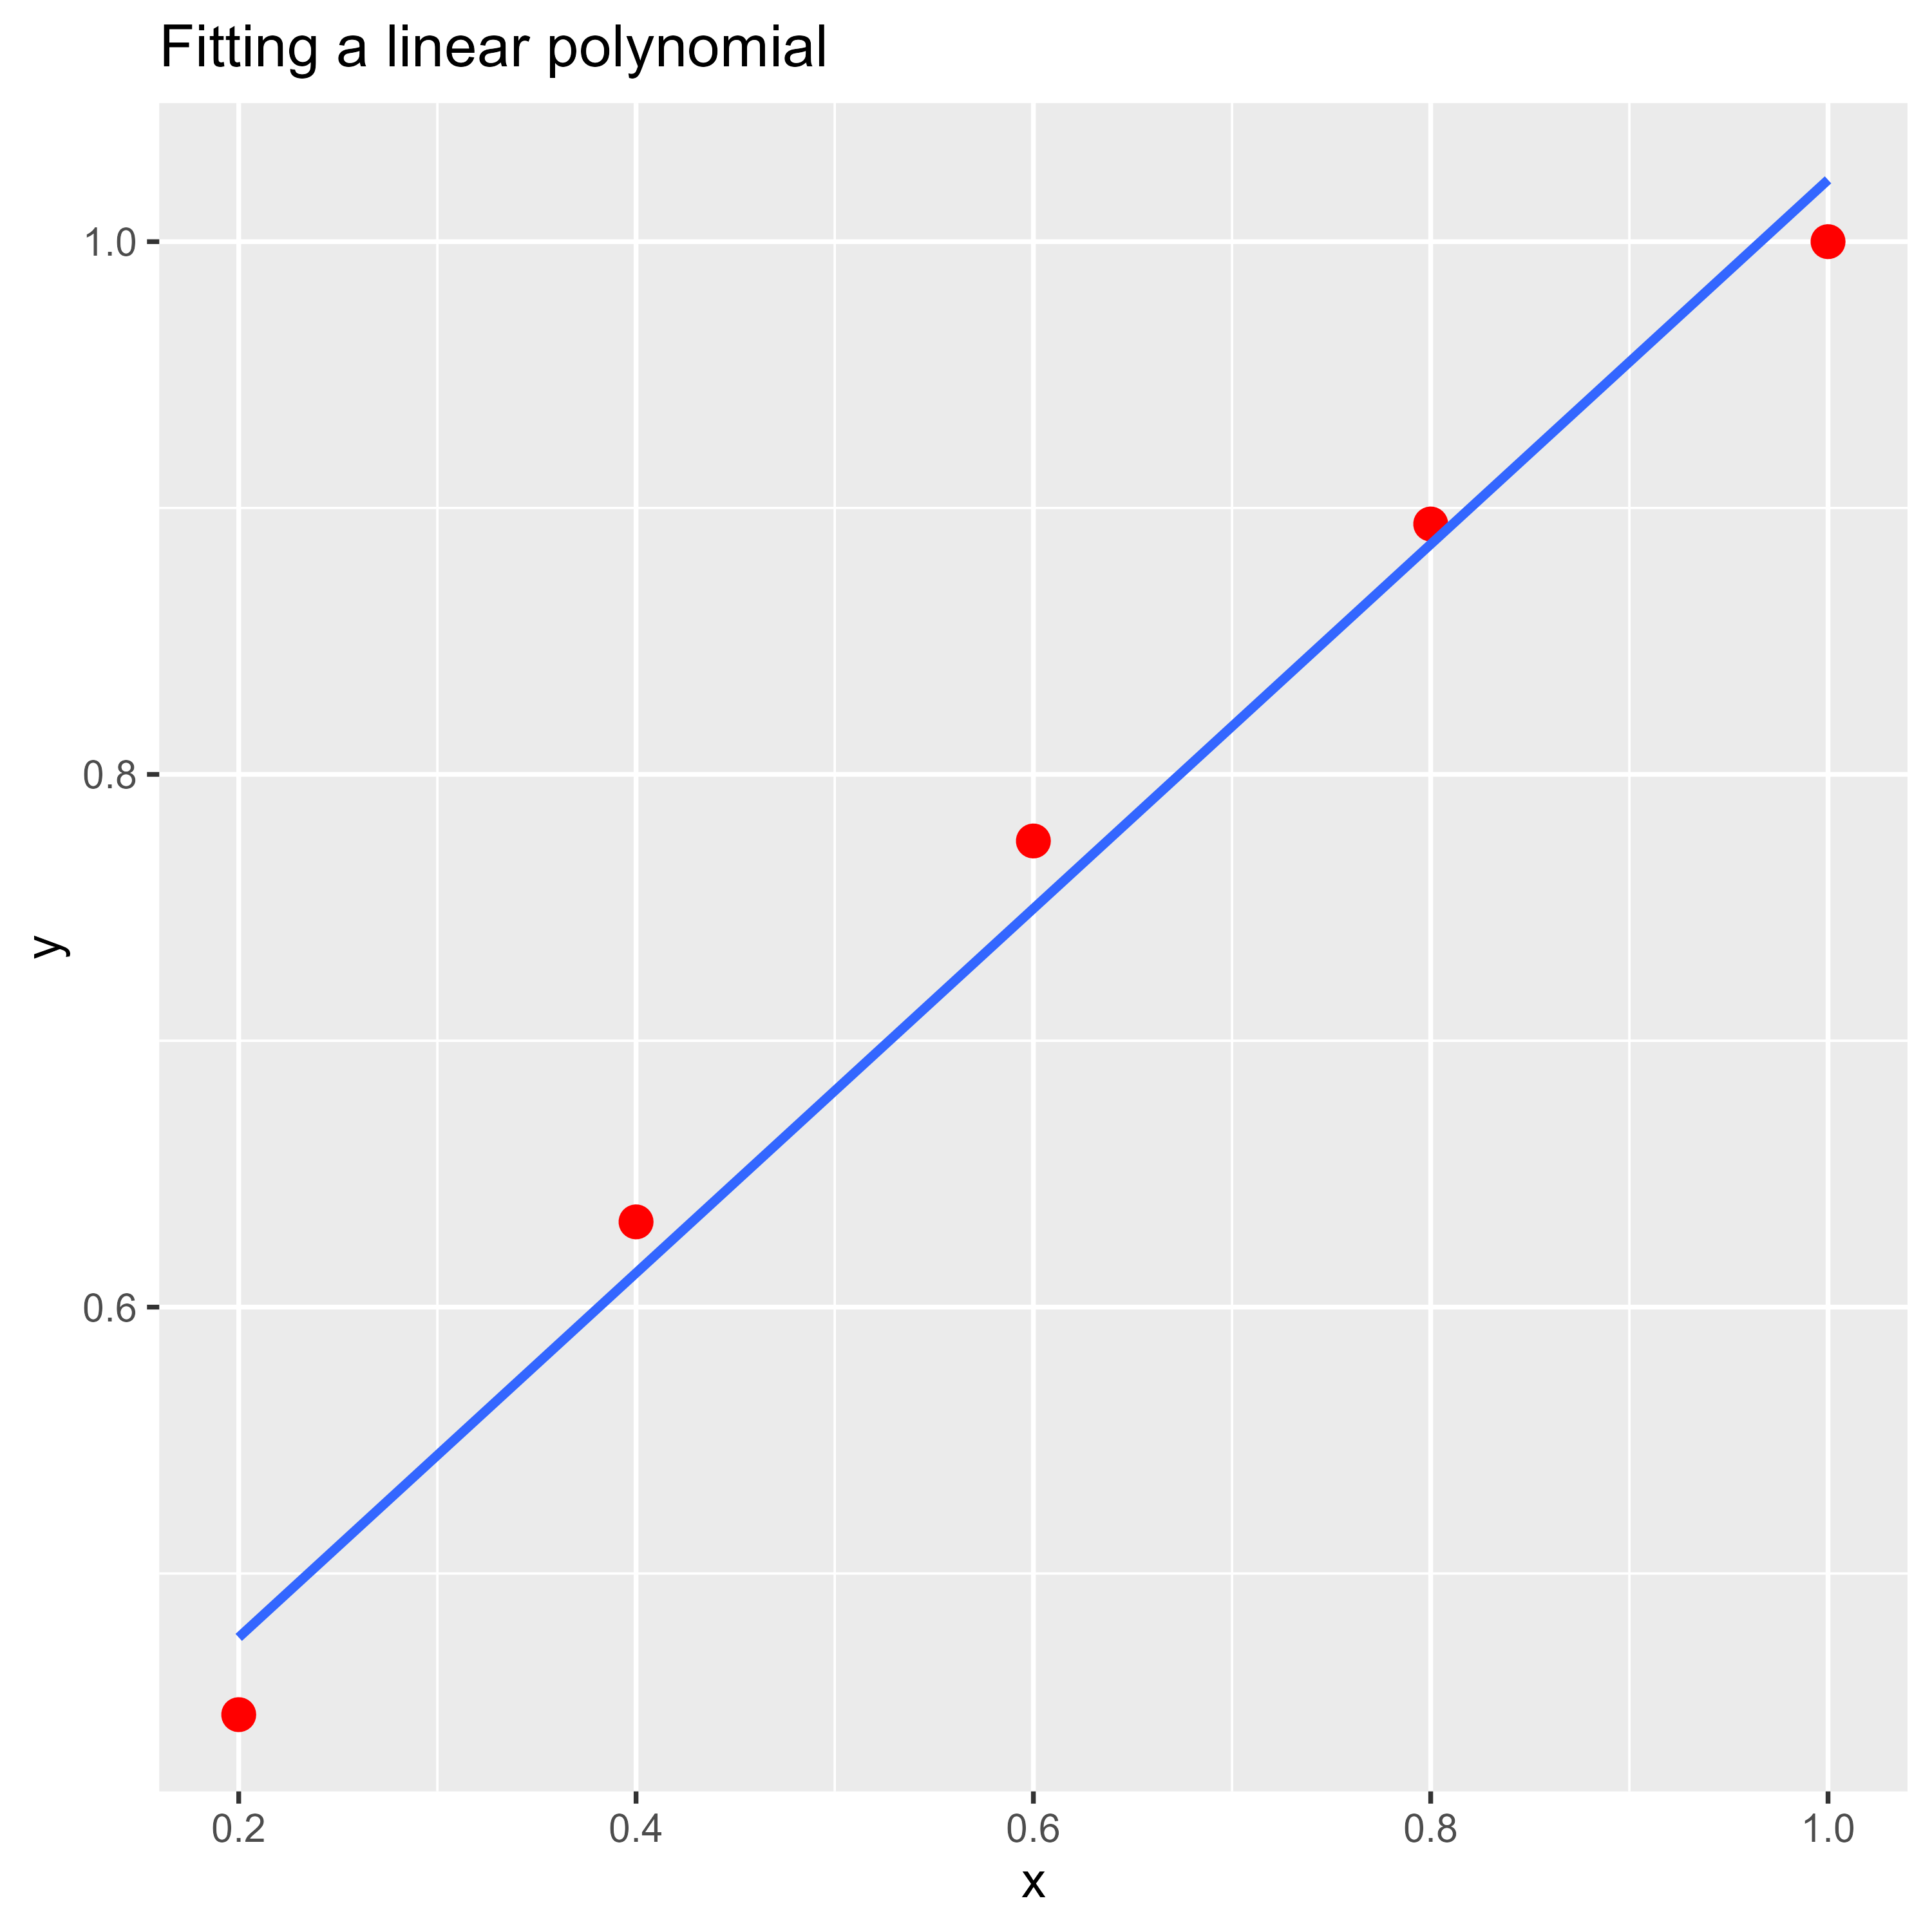
\includegraphics[scale = 0.5]{fit2} & 
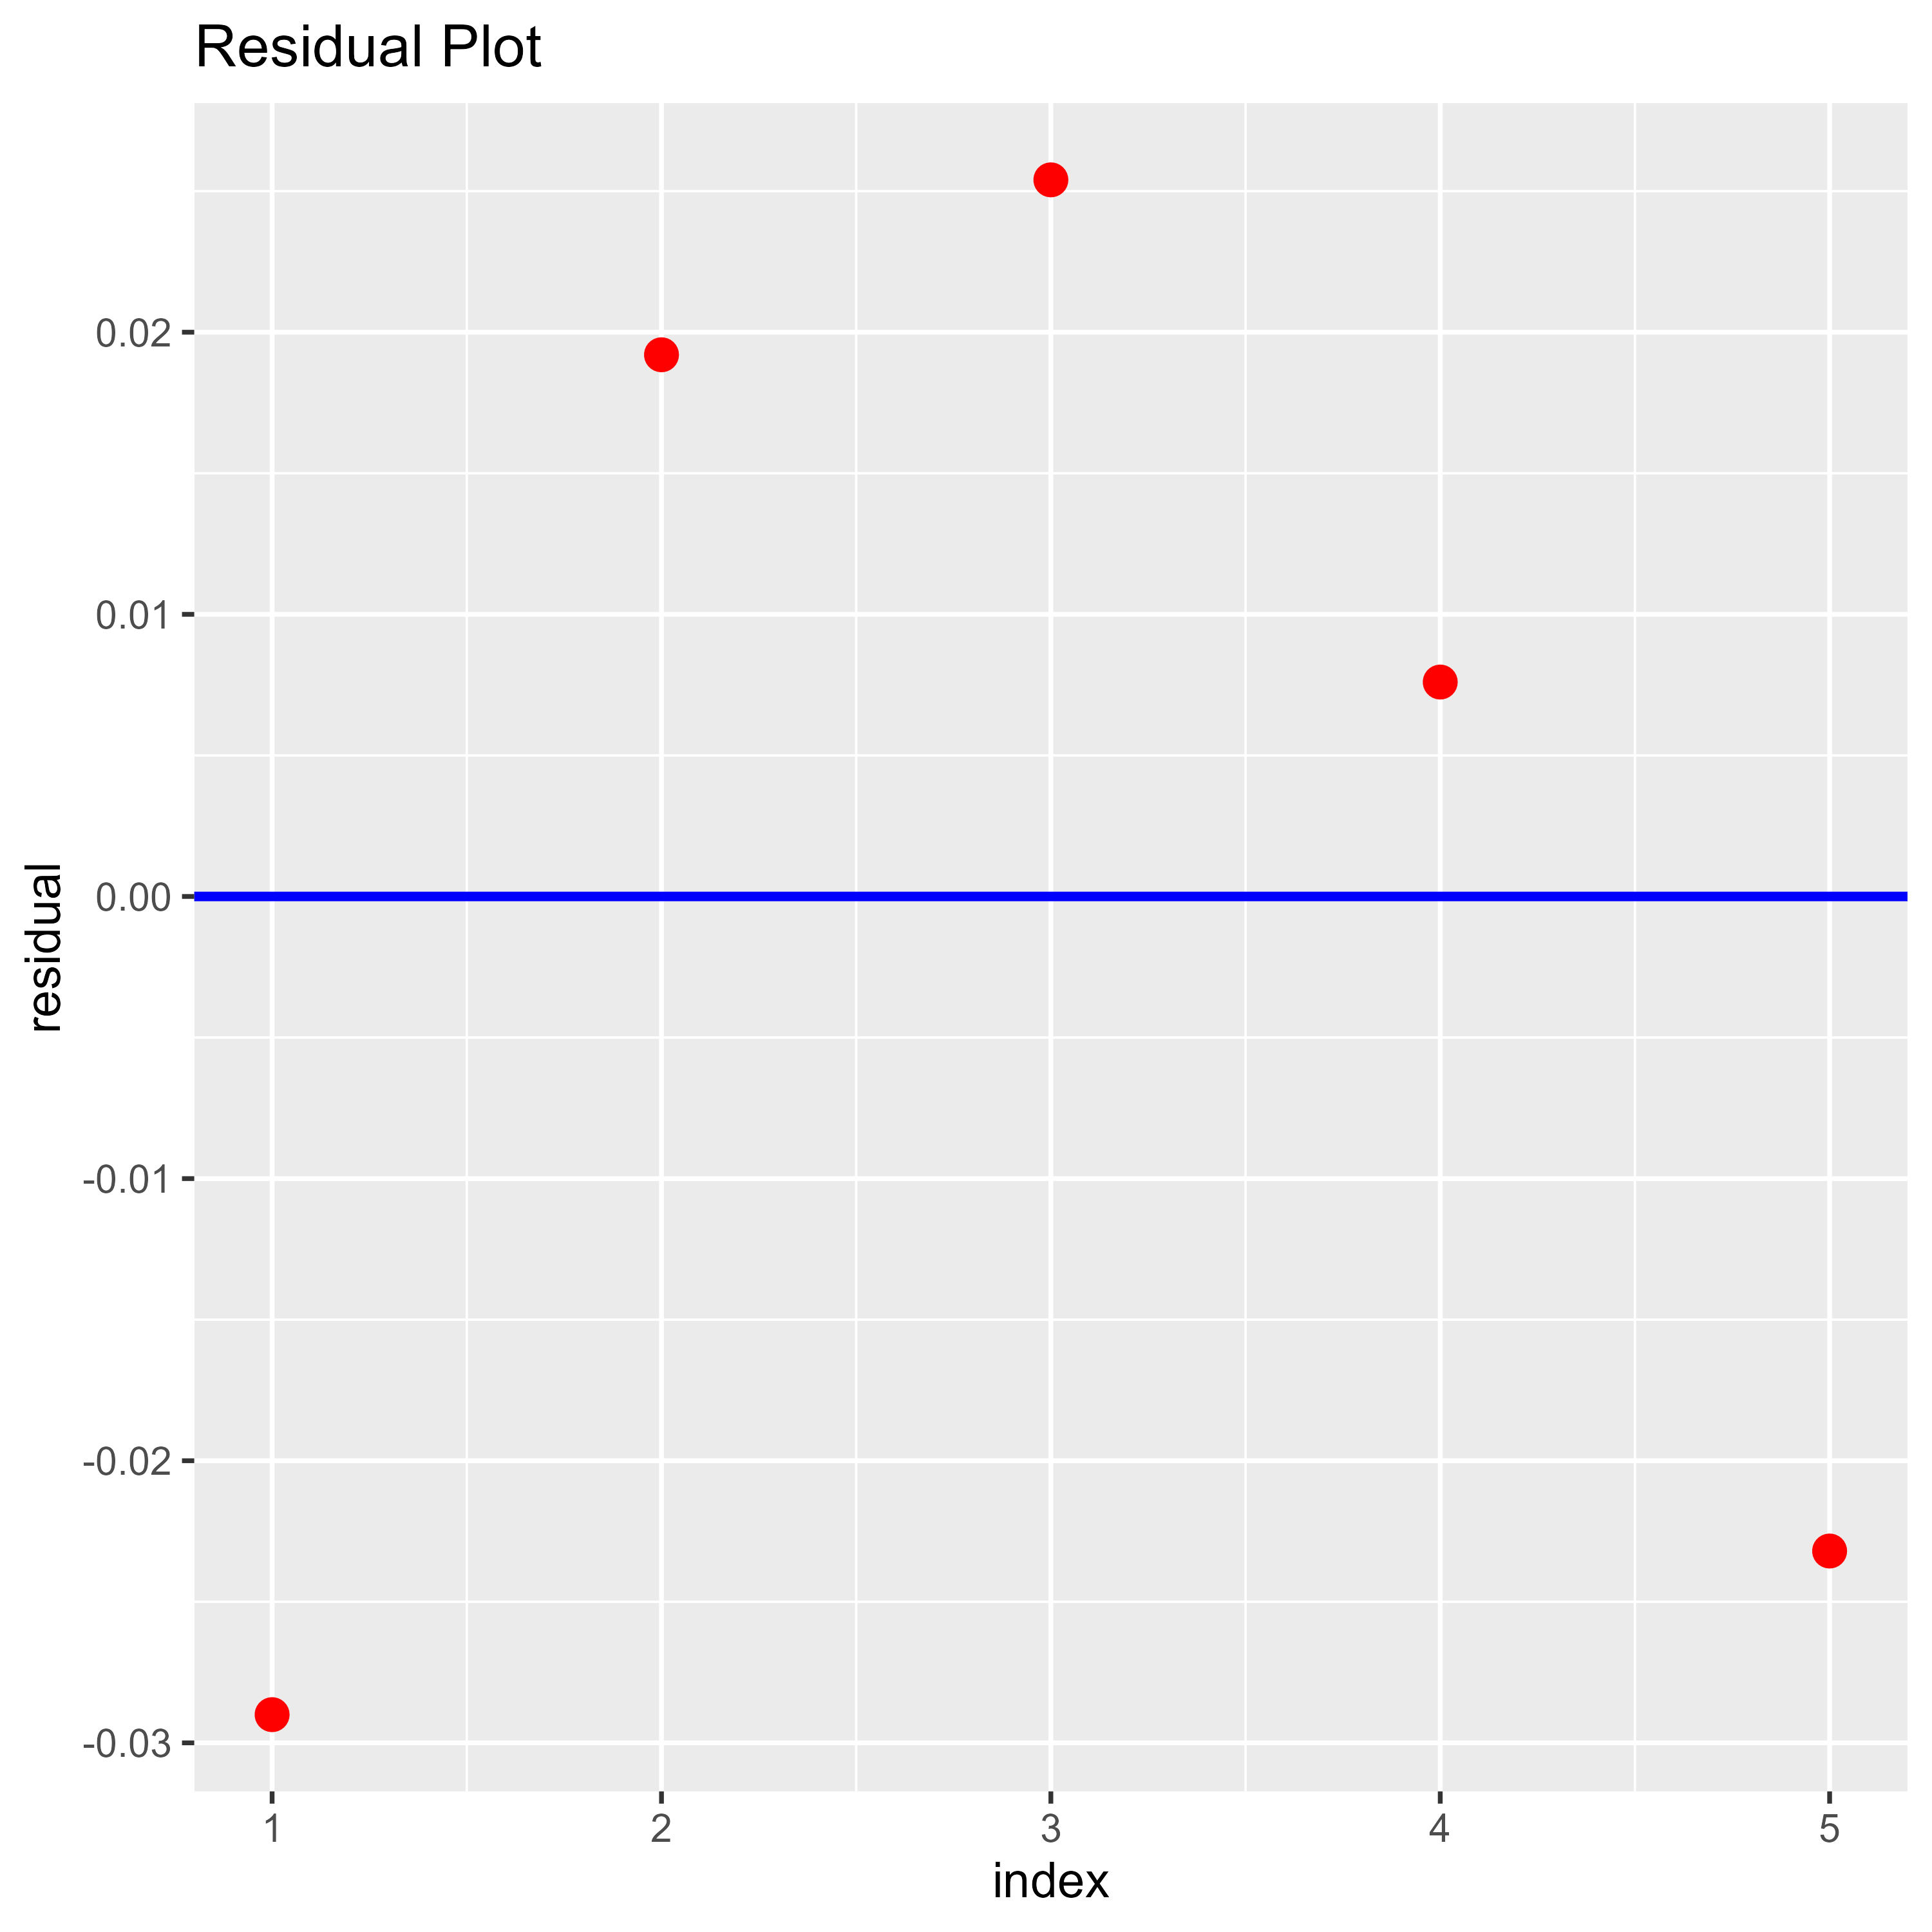
\includegraphics[scale = 0.5]{fit2_residuals}
\end{tabular}
\end{center}
\end{table}


\smallpencil \hspace{0.2cm} Fit a second-degree polynomial to the following data.

\begin{table}[!htbp]
\def\arraystretch{1.5}

\begin{center}
\begin{tabular}{|c|c|c|c|c|c|}

\hline

$x$ & 1 & 2 & 3 & 4 & 5 \\

\hline

$f(x)$ & 2.2 & 4.8 & 8.5 & 14.1 & 20.2 \\

\hline
\end{tabular}
\end{center}

\end{table}

\faArrowAltCircleRight[regular] \hspace{0.2cm} Let $f(x) \approx P_2(x) = a_0 + a_1 x + a_2 x^2$.

\begin{knitrout}
\definecolor{shadecolor}{rgb}{0.969, 0.969, 0.969}\color{fgcolor}\begin{kframe}
\begin{alltt}
\hldef{df3} \hlkwb{<-} \hlkwd{data.frame}\hldef{(}\hlkwc{x} \hldef{=} \hlnum{1}\hlopt{:}\hlnum{5}\hldef{,}
                  \hlkwc{y} \hldef{=} \hlkwd{c}\hldef{(}\hlnum{2.2}\hldef{,} \hlnum{4.8}\hldef{,} \hlnum{8.5}\hldef{,} \hlnum{14.1}\hldef{,} \hlnum{20.2}\hldef{))}
\end{alltt}
\end{kframe}
\end{knitrout}

\begin{knitrout}
\definecolor{shadecolor}{rgb}{0.969, 0.969, 0.969}\color{fgcolor}\begin{kframe}
\begin{alltt}
\hldef{fit3} \hlkwb{<-} \hlkwd{lm}\hldef{(y} \hlopt{~} \hldef{x} \hlopt{+} \hlkwd{I}\hldef{(x}\hlopt{^}\hlnum{2}\hldef{),} \hlkwc{data} \hldef{= df3)}
\hldef{fit3}\hlopt{$}\hldef{coefficients}
\end{alltt}
\begin{verbatim}
## (Intercept)           x      I(x^2) 
##   0.8200000   0.7157143   0.6357143
\end{verbatim}
\end{kframe}
\end{knitrout}

So, $P_2(x) = 0.82 + 0.7157143 x + 0.6357143 x^2$.

\begin{knitrout}
\definecolor{shadecolor}{rgb}{0.969, 0.969, 0.969}\color{fgcolor}\begin{kframe}
\begin{alltt}
\hldef{df3} \hlopt
  \hlkwd{ggplot}\hldef{(}\hlkwd{aes}\hldef{(}\hlkwc{x} \hldef{= x,} \hlkwc{y} \hldef{= y))} \hlopt{+}
  \hlkwd{geom_point}\hldef{(}\hlkwc{col} \hldef{=} \hlsng{"red"}\hldef{,} \hlkwc{size} \hldef{=} \hlnum{3}\hldef{)} \hlopt{+}
  \hlkwd{geom_smooth}\hldef{(}\hlkwc{method} \hldef{=} \hlsng{"lm"}\hldef{,} \hlkwc{formula} \hldef{= y} \hlopt{~} \hldef{x} \hlopt{+} \hlkwd{I}\hldef{(x}\hlopt{^}\hlnum{2}\hldef{),} \hlkwc{se} \hldef{=} \hlnum{FALSE}\hldef{)} \hlopt{+}
  \hlkwd{labs}\hldef{(}\hlkwc{title} \hldef{=} \hlsng{"Fitting a quadratic polynomial"}\hldef{)}
\end{alltt}
\end{kframe}
\end{knitrout}



\begin{knitrout}
\definecolor{shadecolor}{rgb}{0.969, 0.969, 0.969}\color{fgcolor}\begin{kframe}
\begin{alltt}
\hldef{fit3_residuals} \hlkwb{<-} \hlkwd{data.frame}\hldef{(}\hlkwc{index} \hldef{=} \hlnum{1}\hlopt{:}\hlnum{5}\hldef{,} \hlkwc{residual} \hldef{= fit3}\hlopt{$}\hldef{residuals)}

\hldef{fit3_residuals} \hlopt
  \hlkwd{ggplot}\hldef{(}\hlkwd{aes}\hldef{(}\hlkwc{x} \hldef{= index,} \hlkwc{y} \hldef{= residual))} \hlopt{+}
  \hlkwd{geom_point}\hldef{(}\hlkwc{col} \hldef{=} \hlsng{"red"}\hldef{,} \hlkwc{size} \hldef{=} \hlnum{3}\hldef{)} \hlopt{+}
  \hlkwd{geom_hline}\hldef{(}\hlkwc{yintercept} \hldef{=} \hlnum{0}\hldef{,} \hlkwc{col} \hldef{=} \hlsng{"blue"}\hldef{,} \hlkwc{linewidth} \hldef{=} \hlnum{1}\hldef{)} \hlopt{+}
  \hlkwd{labs}\hldef{(}\hlkwc{title} \hldef{=} \hlsng{"Residual Plot"}\hldef{)}
\end{alltt}
\end{kframe}
\end{knitrout}



\newpage

\begin{table}[!htbp]
\def\arraystretch{1.5}

\begin{center}

\begin{tabular}{cc}

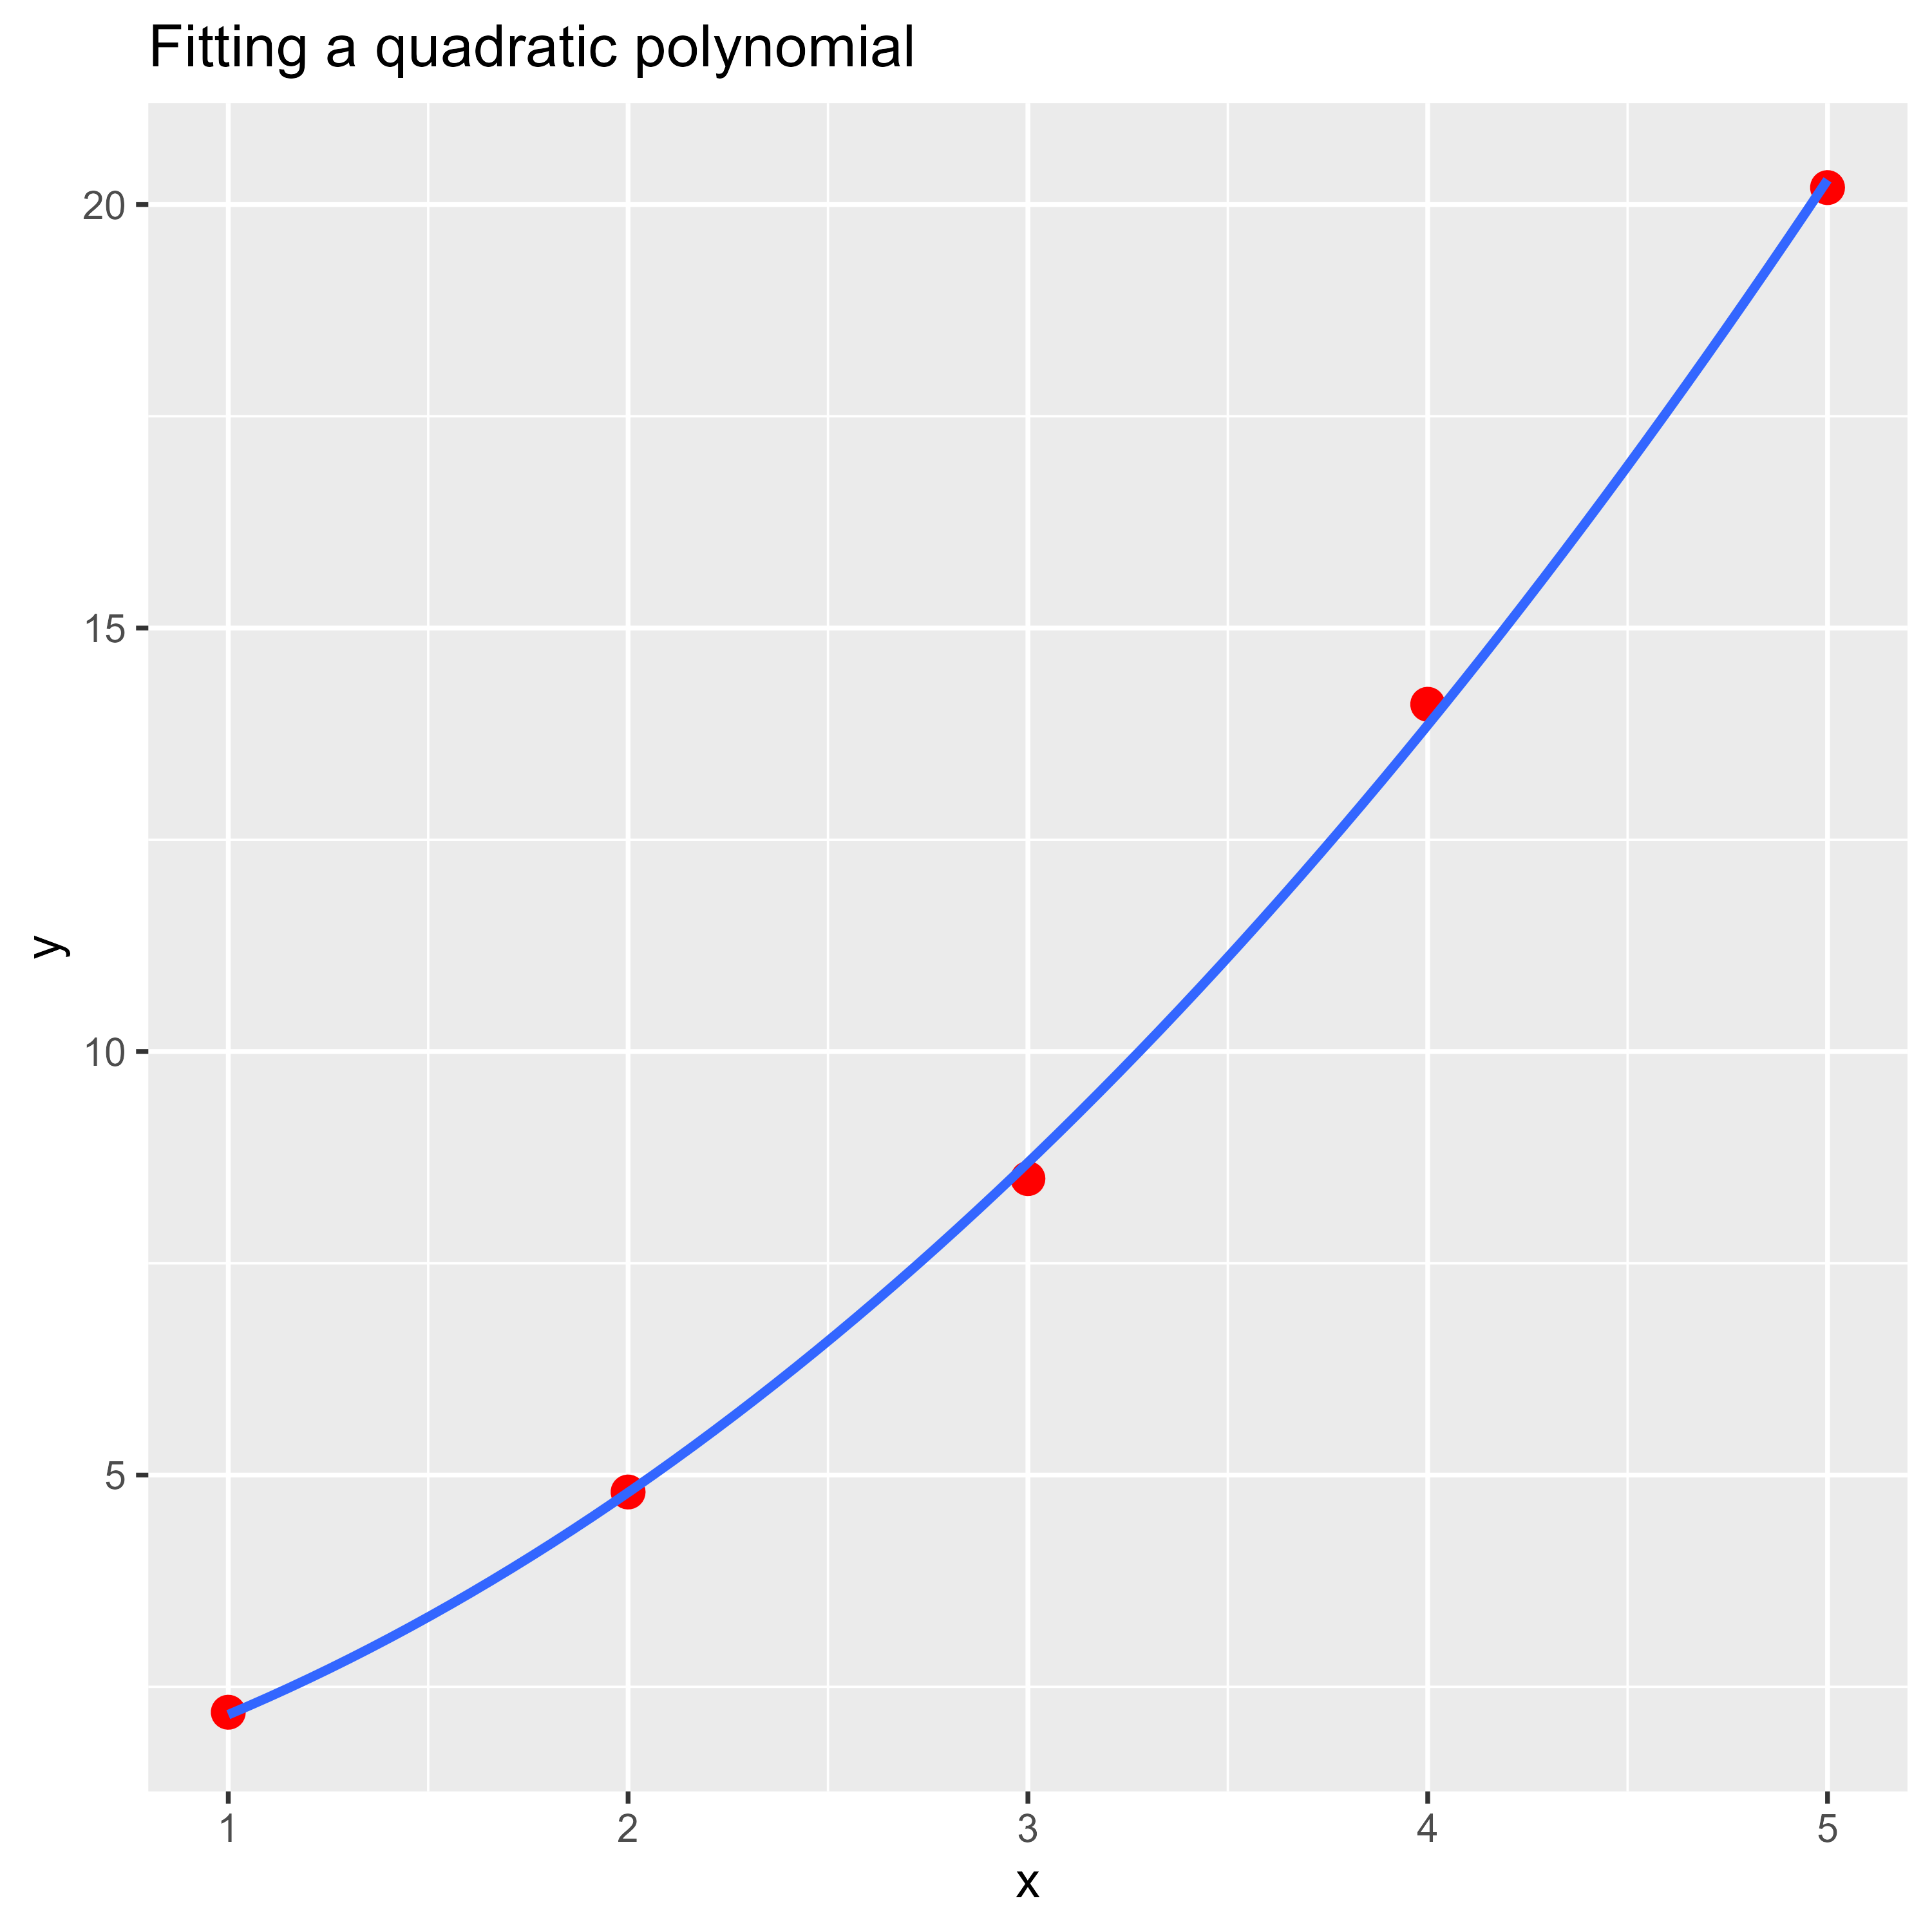
\includegraphics[scale = 0.5]{fit3} & 
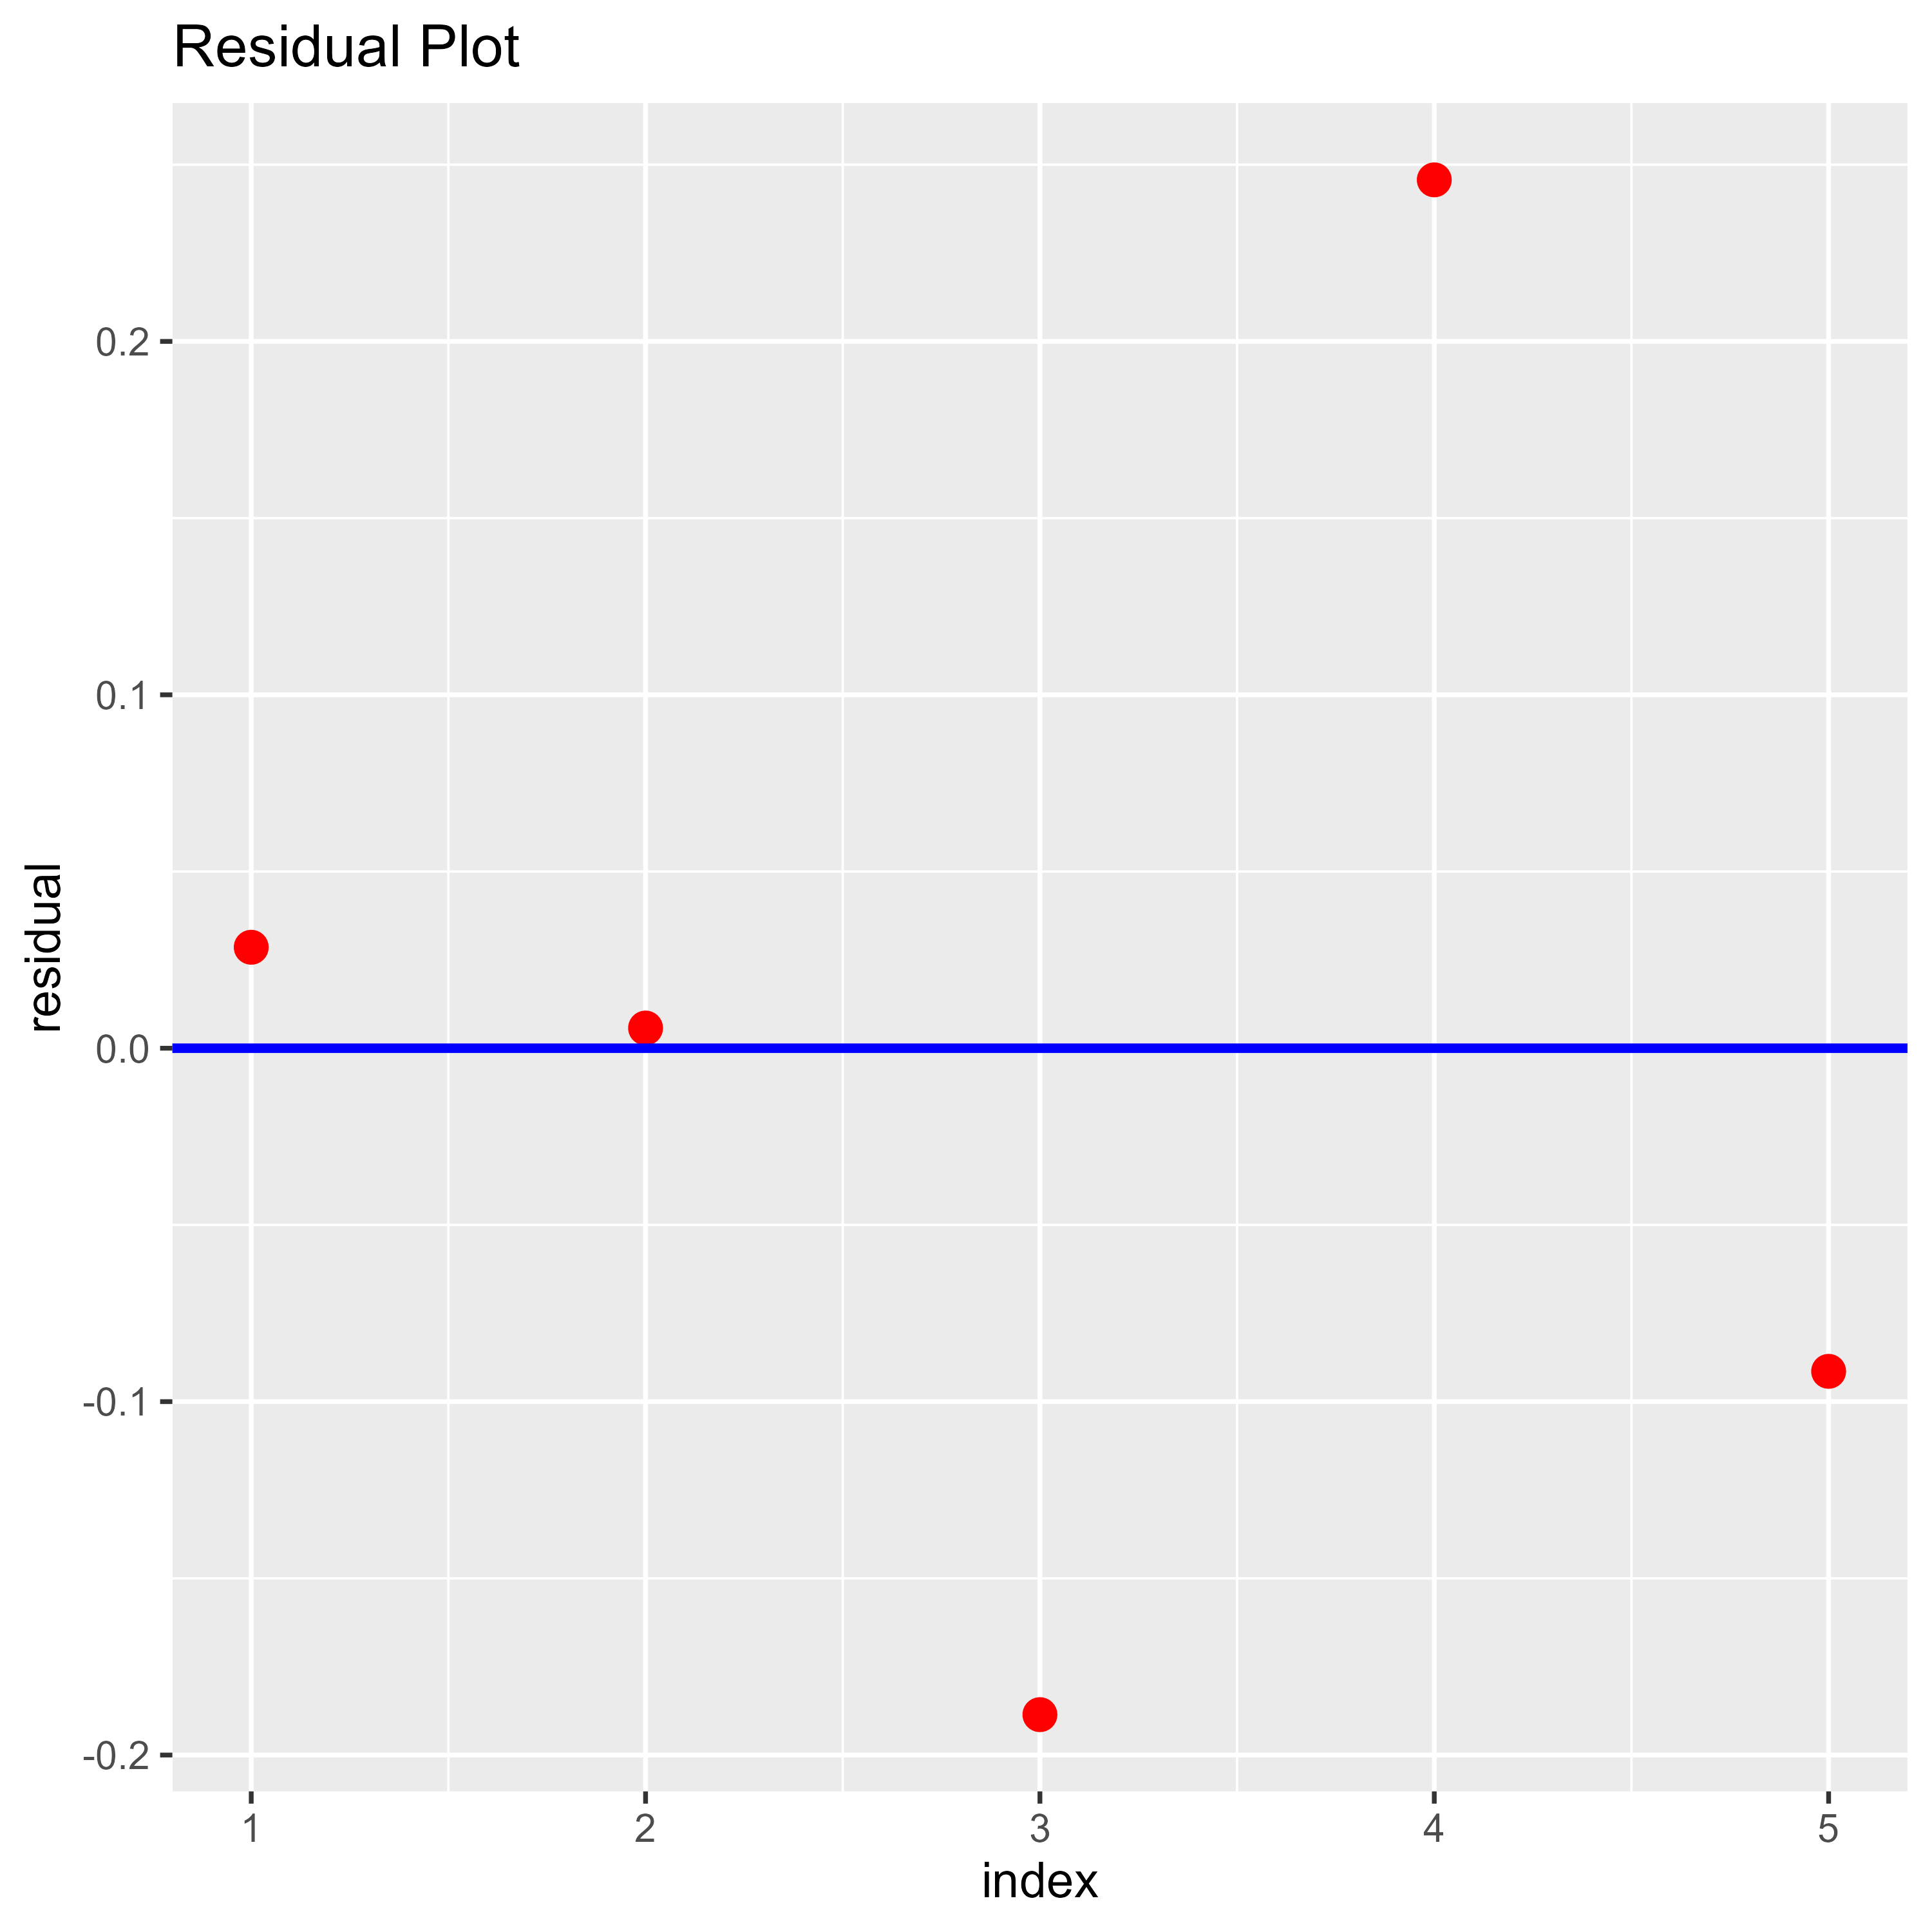
\includegraphics[scale = 0.5]{fit3_residuals}
\end{tabular}
\end{center}
\end{table}



\end{document}
